\section{Approach}
\label{sec_approach}
This section presents our proposed overall approach. It first gives an overview. Then, it describes how to detect the metamodel changes and how to trace their impacts until the tests and map them. Finally, it details our prototype implementation. 




\subsection{Overview}

\red{The overall objective of our approach is to help developers in checking the behavioral correctness of the code co-evolution when metamodels evolve, as the co-evolution may be done incorrectly or in an incomplete way (i.e., referred to as partial co-evolution in \cite{le2021untangling,zaidman2011studying}). 
Several ways exist, such as using formal methods, manual code review, or unit tests, etc. 
%Our assumptions and contribution is to rely on the tests as a mean to check the behavioral correctness of the code co-evolution, similarly as in a regression testing method \cite{leung1989insights,yoo2012regression,wong1997study}. At the very least, it can help to pinpoint to the developers where to start investigating possible incorrect code co-evolution (e.g., passing test that then fails). 
Our scope lies in tracing the impact of the metamodel changes till the tests and rely on them as an indicator for behavioral correctness of the code co-evolution, similarly as in a regression testing method \cite{leung1989insights,yoo2012regression,wong1997study}. Our vision is rather than letting the developers execute all test suite in both versions and manually analyzing them, we can reduce the set of tests to be analyzed to the only minimum necessary one. Thus, saving effort and time for developers.}  

%As depicted in 
Figure \ref{fig:appraoch} depicts the overall approach workflow. We first compute the difference between the two metamodel versions each of them having a generated code and an additional code (step {\small\boxed{1}}). In the original version, the additional code is the impacted one, and in the evolved version, the additional code is the co-evolved one. 
After that, we run the impact and the test tracing analysis to link the metamodel changes to the impacted and co-evolved code and their respective tests (step {\small\boxed{2}}). Therefore, a developer can run the traced tests before and after the code co-evolution to check their behavioral correctness. Finally, to ease this task, we map the traced tests and execute them to report them back in a form of a diagnostic to the developers for an easier in-depth analysis of the effect of metamodel evolution rather than analyzing the whole test suite (step {\small\boxed{3}}). 
\blue{Therefore, in a nutshell, there are no particular preconditions to our approach except having available code and tests from both before and after co-evolution along with the delta of the metamodel changes.} 


\begin{figure*}[tb]
\centering
% \hspace*{-2em}
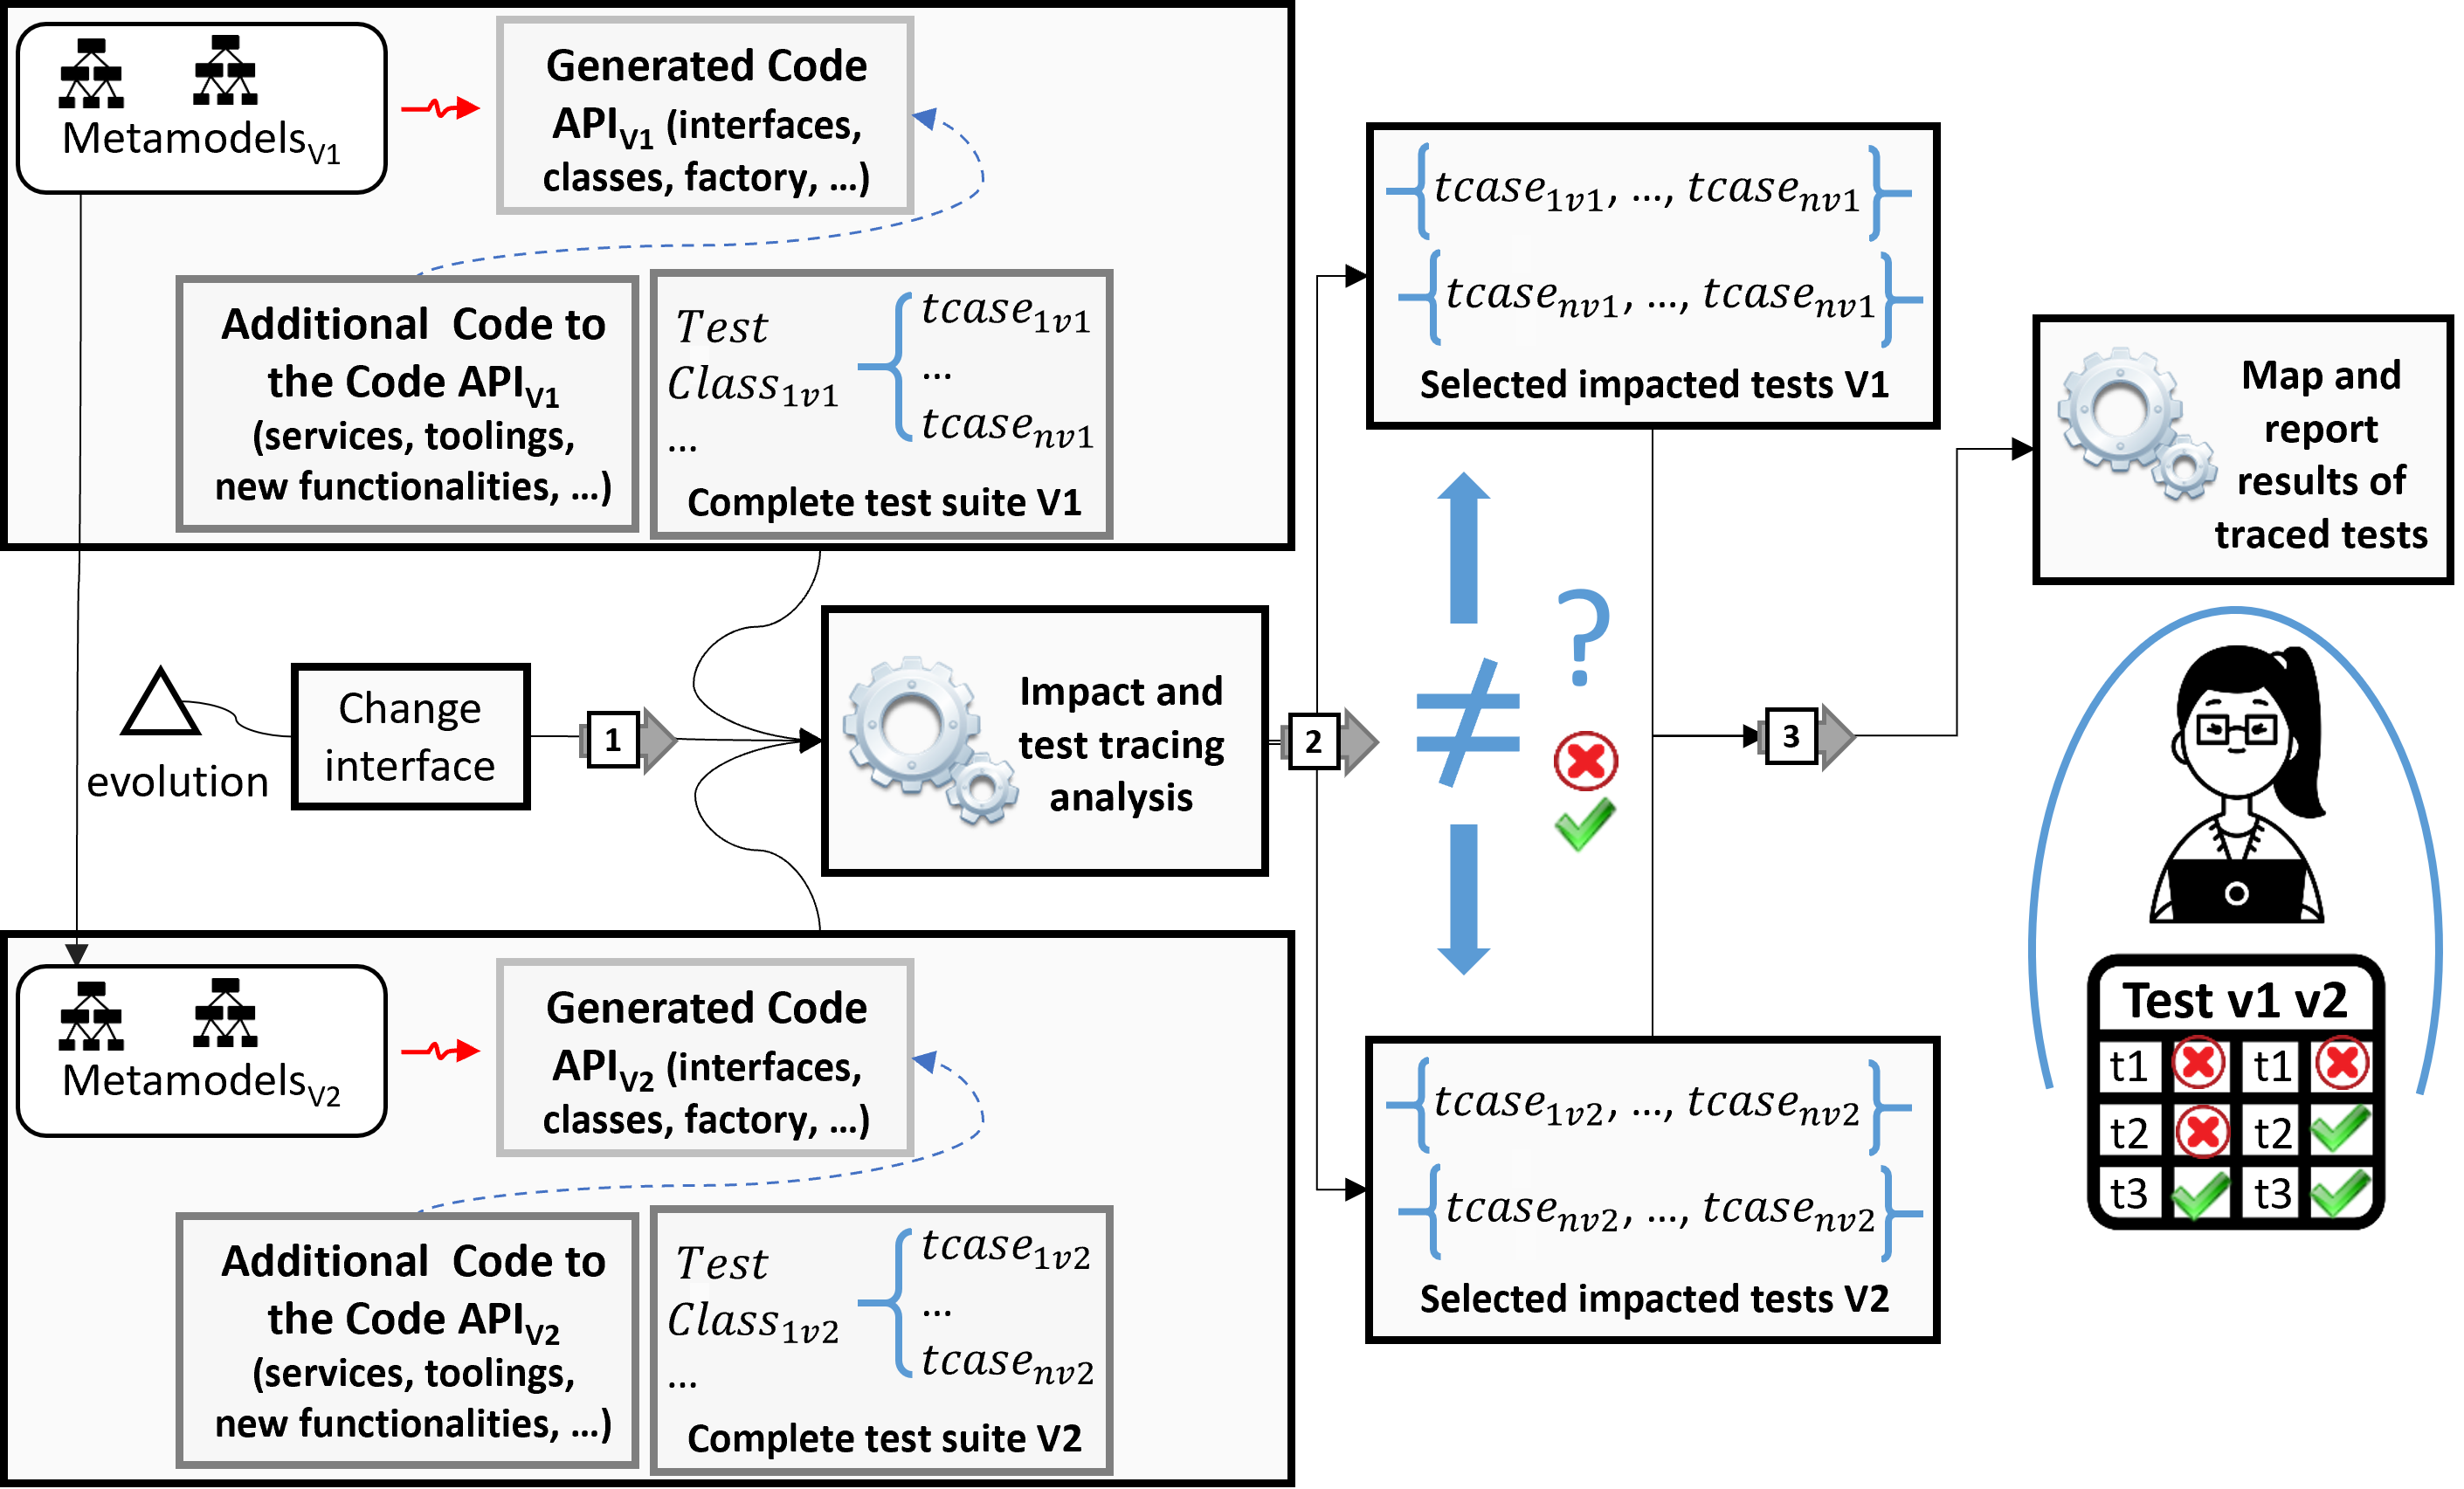
\includegraphics[width=1\textwidth]{./pics/chapter2pics/OverallApproachV2.png}
\caption{Overall approach}
\label{fig:appraoch}
%\vspace{-5mm}
\end{figure*}


\subsection{Detection of metamodel Changes}\label{sec:changes}

%One of the intrinsic property of software artifacts is its continuous evolution~\cite{mens2008introduction}. Metamodels are no different and are meant to evolve. 
Software artifacts continuously evolve over time~\cite{mens2008introduction}.
As any artifact, metamodels evolve as well. 
%Due to many reasons, the metamodel is meant to evolve. 
Two types of changes are known and considered in the literature for metamodel evolution: \emph{atomic} and \emph{complex} changes \cite{Herrmannsdoerfer2011}. 
Atomic changes are additions, removals, and updates of a metamodel element. Complex changes consist of a sequence of atomic changes combined together~\cite{vermolen_reconstructing_2012,khelladi2015detecting}. For example, move property is a complex change where a property is moved from a source class to a target class. This is composed of two atomic changes: delete a property and add a property \cite{Herrmannsdoerfer2011}. 
%Many approaches in the literature \cite{Alter2015, williams2012searching,cicchetti_managing_2009,langer_posteriori_2013,vermolen_reconstructing_2012,Khelladi2016} exist to detect metamodel changes between two versions.
Several existing approaches allow to automatically detect metamodel changes between two versions, such as \cite{Alter2015, williams2012searching,cicchetti_managing_2009,langer_posteriori_2013,vermolen_reconstructing_2012,Khelladi2016}.

In this work, we use an interface specification of changes {\small\boxed{1}} that is a connection layer to our test tracing approach with the existing change detection approaches. It basically defines each metamodel change as a class with its necessary information. Therefore, in practice, any detection approach \cite{Alter2015, williams2012searching,cicchetti_managing_2009,langer_posteriori_2013,vermolen_reconstructing_2012,Khelladi2016} can be integrated by bridging its changes to our interface and the rest of our approach can be performed independently. 
%In the rest of this work, we focus on code co-evolution. We suppose that we have the metamodel changes and their information as input using the changes detection interface. 


% Please add the following required packages to your document preamble:
% \usepackage{multirow}
% \usepackage[table,xcdraw]{xcolor}
% If you use beamer only pass "xcolor=table" option, i.e. \documentclass[xcolor=table]{beamer}
%multiple cells \multicolumn{2}{c}{text}
\begin{table*}[t]
\caption{List of metamodel changes and how they are traced up to the tests in the original and evolved versions. }
\label{tab:changes}
\centering
\resizebox{14cm}{!} {
 \hspace*{-3em}
\begin{tabular}{lcc}
\toprule
                                    & \multicolumn{2}{c}{Tests treatment} \\ \cmidrule{2-3}
\multicolumn{1}{c}{\multirow{-2}{*}{Metamodel changes}} & In original version (V1)            & In evolved version (V2)            \\ \midrule
$\diamond$ Delete property \emph{p} in class \texttt{C}       &   Search for usages of \emph{p} in \texttt{C}                &        \emph{n/a}          \\ \midrule
$\diamond$ Delete class \texttt{C}          &   Search for usages of \texttt{C}               &      \emph{n/a}            \\ \midrule

$\diamond$ Add property \emph{p} in class \texttt{C}     &        \emph{n/a}  & Search for  usages of\emph{p} in \texttt{C}         \\ \midrule
$\diamond$ Add class \texttt{C}     &      \emph{n/a}       &   Search for usages of \texttt{C}                         \\ \midrule


$\diamond$ Rename element \emph{e} to \emph{e'} in class \texttt{C}	           &  Search for usages of \emph{e} in \texttt{C}    & Search for usages of \emph{e'} in \texttt{C}                \\ \midrule

\begin{tabular}[c]{@{}l@{}}$\diamond$ Change multiplicity of property \\ \emph{p} in class \texttt{C} \end{tabular}           &        \multicolumn{2}{c}{Search for usages of \emph{p} in \texttt{C}}           \\ \midrule

\begin{tabular}[c]{@{}l@{}}$\diamond$ Change type of property \emph{p}  \\from \texttt{S} to \texttt{T}\end{tabular}           &      \multicolumn{2}{c}{Search for usages of \emph{p} in \texttt{C}}     \\ \midrule
           
\begin{tabular}[c]{@{}l@{}}$\diamond$ Move property $p_{i}$ from \\ class \texttt{S} to \texttt{T} through \emph{ref}\\
%$\diamond$ Extract class \texttt{S} to \texttt{T} \\with properties $p_{1},...,p_{n}$ \\ \red{through \emph{ref}}\\
$\diamond$ Extract class of properties $p_{1},$\\$...,p_{n}$ from \texttt{S} to \texttt{T} through \emph{ref}\end{tabular}           &     Search for usages of all $p_{i}$ in \texttt{S}             &      Search for usages of all $p_{i}$ in \texttt{T}             \\ \midrule

\begin{tabular}[c]{@{}l@{}}$\diamond$ Push property $p_{i}$ from \\class \texttt{Sup} to \texttt{Sub$_{1}$},...,\texttt{Sub$_{n}$}\end{tabular}           &    Search for usages of all $p_{i}$ in \texttt{Sup}              &    Search for usages of all $p_{i}$ in all \texttt{Sub$_{i}$}               \\ \midrule

\begin{tabular}[c]{@{}l@{}}$\diamond$ Pull property $p_{i}$ from \\classes \texttt{Sub$_{1}$},...,\texttt{Sub$_{n}$} to \texttt{Sup}  \end{tabular}           &     Search for usages of all $p_{i}$ in all \texttt{Sub$_{i}$}             &    Search for usages of all $p_{i}$ in \texttt{Sup}                 \\ \midrule
    
\begin{tabular}[c]{@{}l@{}}$\diamond$ Inline class \texttt{S} to \texttt{T} \\with properties $p_{1},...,p_{n}$\end{tabular}           &      Search for usages of all $p_{i}$ in \texttt{S}               &      Search for usages of all $p_{i}$ in \texttt{T}          \\ %\midrule

%&                  &                  \\ 
                                    
                                    \bottomrule                 
\end{tabular}
}
\end{table*}

%\red{here add a table or an item list of changes we handle}

\blue{}In practice, we focus on the impacting metamodel changes that will require co-evolution of the code and not on the non-impacting changes. For example, a delete change or a change of type will impact the code and possibly its behavior that can be observed with its tests. 
However, addition changes, although \red{non-breaking}, can be traced back to their newly added tests. Thus, we also consider them to observe their behavior.
%as new metamodel elements are added in the evolved version, we also consider addition changes, although non-impacting, to trace them back to their newly added tests and observe their behavior. 
The list of metamodel changes \cite{iovino2012impact,cicchetti_managing_2009} we consider for tracing their impact up to the tests is as shown in the first column of Table \ref{tab:changes}. 

%Table \ref{tab:changes} depicts the metamodel changes we considered including all impacting changes as well as addition changes that are not necessary breaking, yet, still leading to added tests in the evolved version. 
For each version of the tests, we use different information provided by each metamodel change, depending on whether we are tracing the impacted tests in the original or the evolved versions. Columns 2 and 3 of table \ref{tab:changes} detail the treatments of each metamodel change in the original and evolved versions. For example, for a rename element \emph{e} to \emph{e'}, we search for \emph{e} and \emph{e'}, respectively, in the original and evolved versions. Similarly, for the other changes, such as Move, Pull, Push, etc. where the source and target classes are different in the original and evolved versions. Only the impact of delete changes is searched in the original version, while the impact of addition changes is only searched in the evolved version. 





\begin{comment}   

The list of impacting metamodel changes \cite{iovino2012impact,cicchetti_managing_2009} we consider for tracing the tests is as follows: 
\emph{1)} Delete property \emph{p} in a class \texttt{C}. 
\emph{2)} Delete class \texttt{C}. 3) Rename element \emph{e} in a class \texttt{C}.
\emph{3)} Generalize property \emph{p} multiplicity from a single value to multiple values in a class \texttt{C}.
\emph{4)} Move property \emph{p} from class \texttt{S} to \texttt{T} through a reference \emph{ref}.
\emph{5)} Extract class of properties $p_{1},...,p_{n}$ from \texttt{S} to \texttt{T} through a reference \emph{ref}.
\emph{6)} Push property \emph{p} from super class \texttt{Sup} to sub classes \texttt{Sub$_{1}$},...,\texttt{Sub$_{n}$}.
\emph{7)} Inline class \texttt{S} to \texttt{T} with properties $p_{1},...,p_{n}$.
\emph{8)} Change property \emph{p} type from \texttt{S} to \texttt{T} in a class \texttt{C}.
\end{comment}

\begin{comment}

    %\item[$\diamond$] 
    \item Delete property \emph{p} in a class \texttt{C}.
    \item Delete class \texttt{C}.
    \item Rename element \emph{e} in a class \texttt{C}.
    \item Generalize property \emph{p} multiplicity from a single value to multiple values in a class \texttt{C}.
    \item Move property \emph{p} from class \texttt{S} to \texttt{T} through a reference \emph{ref}.
    \item Extract class of properties $p_{1},...,p_{n}$ from \texttt{S} to \texttt{T} through a reference \emph{ref}.
    \item Push property \emph{p} from super class \texttt{Sup} to sub classes \texttt{Sub$_{1}$},...,\texttt{Sub$_{n}$}.
    \item Inline class \texttt{S} to \texttt{T} with properties $p_{1},...,p_{n}$.
    \item Change property \emph{p} type from \texttt{S} to \texttt{T} in a class \texttt{C}.
\end{comment}

\subsection{Tracing the Impacted Tests}
\label{section: tracing the impacted tests}
\red{}


Our approach traces the impact of metamodel changes up to the test. To do that, we structure the code source to better navigate in it. 
Before starting, we parse the code source including tests and build the Code Call Graph (CCG) at the methods level. It consists of nodes $\mathbb{N}$ that are methods, and edges $\mathbb{E}$ that are calls between methods. 
For a given method, the CCG allows us to retrieve its callers, hence, tracing the call methods recursively up to the tests. %map between the code elements (CE) and their usages in the code (CEU). After that, we link the %, as shown in Table \ref{x}.
After that, we apply Algorithm \ref{algo :impactedTestsDetection} on the built CCG. Overall, for each detected metamodel change, the algorithm computes the list of direct and indirect impacted tests that can be traced to the given metamodel change. 


First, we analyze the AST of the code to identify the code usages of the evolved metamodel element. The information concerning the metamodel element before and after evolution, which is included in the metamodel change (see Table \ref{tab:changes}), allow us to spot the impacted code usages (Line 1). For example, for a rename property \emph{id}, the algorithm will first find its usages, such as \emph{getId()} or \emph{setId()}\footnote{\blue{Note that the knowledge about the generated code elements from the metamodel elements (e.g., getter/setter for EAttribute, class/interface for EClass, etc.) is so far hard-coded in the implementation of Algorithm \ref{algo :impactedTestsDetection}. The mappings must be provided for our approach to be able to trace the tests.}}. 
%
Then, we filter these impacted code usages by keeping only the ones found inside a method declaration. % for example : variable declaration or an If condition clause, etc. 
Let us call the found method declaration using the impacted code \textit{IM()} (Line 5). If \textit{IM()} is a test method, that means that we found a direct impacted test (Line 7). Otherwise, thanks to the CCG, we retrieve \textit{IM()}'s parents \emph{parentsOfIM}, which are all the method declarations invoking IM() (Line 9-17). 
%
Afterwards and recursively, we check each parent of \textit{IM()} if it is a test method or not (Line~14). The process is finished if we reach a method declaration that has no parents in the CCG that is either a test or not, or if the reached method declaration is already treated in the \emph{parentsOfIM}. Therefore, by design, after browsing all the impacted code usages, Algorithm \ref{algo :impactedTestsDetection} traces the list of all impacted tests, without missing any if impacted. \red{It is worth noting that tracing all impacted tests holds syntactically and w.r.t. static semantics. Possible side-effect will require further advanced dynamic analysis and is left for future work.} 
Listing \ref{lis:Modisco_impactedtest_V2} presents an example of an impacted test in the Eclipse Modisco.infra.discovery.benchmark project. 
\red{As described in Section \ref{sec:changes}, we detect that the attribute setTotalExecutionTimeInSeconds is renamed and moved from the class Discovery to the class DiscoveryIteration. After that, Algorithm \ref{algo :impactedTestsDetection} detects the code usage \emph{getDiscoveryTimeInSeconds}. Then, it traces it to the method \emph{test000}. As it has the \emph{@Test} annotation, we conclude that \emph{test000} is an impacted test due to the detected move change. 
%
Note that a test can be impacted by multiple metamodel changes, and one metamodel change can impact many tests. Algorithm \ref{algo :impactedTestsDetection} will detect either cases. 
}

\setulcolor{green} 
\begin{comment}
    

\begin{lstlisting}[language=Java,breaklines=true,mathescape,literate={\-}{}{0\discretionary{-}{}{}},caption=Excerpt of an impacted test in modisco project.\label{lis:Modisco_impacted_test}]
  @Test(timeout = 4000)
  public void test045()  throws Throwable  {
      DiscoveryImpl discoveryImpl0 = new DiscoveryImpl();
      ...    
      assertNull(discoveryIterationImpl0.(*\ul{getDiscoveryErrors()}*));
      assertEquals(0.0, discoveryIterationImpl0.getDiscoveryTimeInSeconds(), 0.01);
      ...
  }
\end{lstlisting}
\end{comment}
%assertTrue(discoveryIterationImpl0.eDeliver());

%we try to match the different code usages of the metamodel element in the code by finding the first impacted code elements and their usages (Lines 3-4).

%for example, for a rename property \emph{id}, the algorithm will first find its usages, such as \emph{getId()}. %These are the Then, if the usage is in a test case (i.e., test method) we add the test to the selected ones to be handled (Lines 6-7). Otherwise, we continue with the usages recursively between methods calls and check if the next parent method call is a test or not (Lines 8-11). Finally, we continue until all the CCG has been completely treated. The process is repeated on all changes by calling the \ref{algo :impactedTestsDetection} on the impacting metamodel changes of section \ref{sec:changes}. 
% Therefore, by design, if there is a set of impacted tests by % a metamodel change, Algorithm \ref{algo :impactedTestsDetection} will be able to trace them and present them for the developers.
%Our Algorithm \ref{algo :impactedTestsDetection} finds the as an entry point in the CCG the code element usages for the metamodel element that is changed. 
%Then, finds its callings methods recursively until reaching a test or not. 
 


%Then, we parse the code to find the different pattern usages of each metamodel element in the code. 
%After that, we recursively search for its usages in the code call graph until reaching the tests. Thus, we end up matching metamodel changes with impacted code methods and their corresponding tests. 



%here explain the pseudo algorithm 

%and explain it 
% todo : format of abv
%Our approach is based on navigating the code call graph containing code elements (CEs). Each code element (CE) is attempt to be linked  with the changes detected between two versions of the metamodel.
%Details
%We start by browsing all the compilation units to compute the graph of code call, it contains all the code elements and their usages in the whole code. 
%For each detected change, we compute the list of  direct and indirect impacted tests with the Algorithm \ref{algo :impactedTestsDetection}. Each code element ( a variable declaration, method invocation or a parameter in a for loop condition for example) is analyzed. If it is used in a test method, we say that the code element is directly impacted by the change. The detected test method is then added to the output result. Otherwise, we fetch the list of usages of the code element. Then , we check for each usage, if it is contained in a test method or not. If a usage is found inside a test method, we say the the code element is indirectly impacted by the change.

% mention in the approach schema that we generate a report 
%The process is repeated until we reach a code element that does not have any usages or all the code call graph has been completely treated.


%here since we will not calculate the precision and recall, maybe we can make the argument of by design we trace all paths to tests to not miss any, so kind of by deisgn we will find all tests

 \begin{comment}
    
\begin{table}[t]
	%\vspace{-1.5em}
	\centering
	%\hspace*{-1.5cm}
	\caption{Mapping table used for the impact analysis.}
	%\resizebox{9cm}{!} {
		\begin{tabular}{cc}
			\toprule
			%\begin{tabular}[c]{@{}l@{}}Metamodel Elements\end{tabular}  & 
   \begin{tabular}[c]{@{}l@{}}Code element\end{tabular} & \begin{tabular}[c]{@{}l@{}}usages\end{tabular}\\ \midrule
			%$e_{1}[type, container]$ & 
   $ce_{1}, ... $    & $ceu_{1}, ceu_{2}, ... $ \\ \midrule
			 ... & ... 	  \\ \midrule
			%$e_{n}[type, container]$ & 
   $ce_{m}, ... $    & $ceu_{j}, ceu_{j}, ... $ \\ \bottomrule                  
		\end{tabular}
	%}
	\label{Mappingtable}
	
\end{table}

\end{comment}


%\todo{does this test change syntactically and/or behaviorally between V1 and V2? if so, can we use it as motivating example}

%\subsection{Amplification of tests/assertions??}
%can we do it with dspot?

\subsection{Mapping of impacted tests}

%this would allow to build a summary table between v1 v2 of the mapped table
After having traced the impacted tests, we further assist developers in analyzing the output of our approach. We provide a diagnostic in a form of a visualized report. This report displays the mapping of impacted tests between the original and evolved versions, along with the verdict of their execution (i.e., pass, fail, and error) and the corresponding impacted change. As an input to generate the diagnostic, the developer selects two impacted traced test classes in the original and evolved versions.
%select two test classes that represent the same impacted test class from the first and second versions. 
The mapping between the two sets of test cases for these classes is performed using a state-of-the-art tool, namely GumTree \cite{falleri2014fine}. It parses both test classes into a tree structure to enable the matching of the test cases. Herein, we distinguish three cases, namely:~1) tests that exist in both versions,~2) tests that exist in the original version but not in the evolved one, and~3) tests that exist in the evolved version but not in the original one.
The impacted tests are then executed programmatically using JUnit runner. To facilitate the analysis and the tracing of impacted tests, we include the corresponding impacting metamodel changes in an additional column of the diagnostic report.  

\definecolor{circlegreen}{HTML}{7ed321}
\begin{algorithm}
\caption{Impacted tests detection}\label{algo :impactedTestsDetection}
\begin{algorithmic}[1]
%\textbf{Input :}{codeCallGraph, change}


\Require codeCallGraph, change
%\Ensure $y = x^n$ 
\State impactedUsages $\leftarrow$ match(AST, change)

\State impactedTests $\leftarrow \phi$ 
\For {(impactedUsage $\in$ impactedUsages )}
    
\State \emph{\textcolor{circlegreen}{ \footnotesize{/* Find the method declaration using impactedUsage*/}}}
            
\State IM $\leftarrow$ getIM(impactedUsage, codeCallGraph) 	       
 \If{(isTest(IM))}
                
             \State   impactedTests.add(IM) 	\emph{\textcolor{circlegreen}{/*If not already added*/}}
    
  \Else
            
             \State parentsOfIM $\leftarrow$ getParents(IM, codeCallGraph)
              
            \State  nextRound.add(parentsOfIM)
                        
            \While{(nextRound.hasNewIMs())}
                    
                    \State    IM $\leftarrow$ nextRound.get()
                        
                        
                            \If{(isTest(IM)}
                            
                             \State  impactedTests.add(IM)\emph{\textcolor{circlegreen}{/*If not already added*/}}
                            
                            \Else 
                            
                            \State  parentsOfIM $\leftarrow$ getParents(IM, codeCallGraph)
                             
                           \State   nextRound.add(parentsOfIM) 
                            \EndIf


                        
                    
            \EndWhile
            \EndIf
\EndFor
\end{algorithmic}
\end{algorithm}


\red{Figure \ref{fig:toolView} illustrates a screenshot of the test tracer report on a toy example "Employee Management Project". After selecting the class of tests that have been traced before code co-evolution, and the class of tests that have been traced after code co-evolution, the user clicks on "Map tests" to display the table of mapped tests with their verdict of execution.
 To illustrate the verdict of the test execution, we made: the passing test in \textcolor{green}{green}, the failing test in \textcolor{blue}{blue}, and erroneous tests in \textcolor{red}{red}. For example, the change "Delete Class Contact" impacts two tests, test11 which passes, and test06 which fails. The verdict of the execution of the tests has no relation with the change itself but with the test that uses the code elements impacted by the metamodel change. Those tests do not exist anymore in the evolved version since the class Contact is absent and cannot be tested anymore.}

%The change "Contact Delete Class" impacts two tests in V1( before code co-evolution): test11, and test06, and no test is impacted by this change in V2 ( after code co-evolution) because the class contact does not exist anymore and cannot be used in the evolved version of the code.
%Even though test11 and test06 are impacted by the same change, that does not imply that they must have the same verdict. It depends on the code that used the deleted class.
%in fig \ref{}, we show the three possible cases? scenarios : tests exist in both version, a test that exist in the first version but not in the second one, and the last case, a test that exist in the second version but not in the first version.


\subsection{Tool implementation}

We implemented our solution as an Eclipse Java plugin handling Ecore/EMF metamodels and their Java code. %a state-of-the-art
We rely on our approach \cite{khelladi2015detecting} to perform the detection of the metamodel changes bridged with the change interface. 
The test tracing, technically, consists of parsing the java code and manipulating its AST using JDT eclipse plugin\footnote{Eclipse Java development tools (JDT): \url{https://www.eclipse.org/jdt/core/}} to construct the Code Call Graph (CCG). After that, we navigate within the methods calls until we either reach a test or not. Finally, for each impacted \emph{TestClass}, we create a copy \emph{TestClass\_Impacted} where we only include the impacted traced test cases. The developer can then launch the traced tests in both the original and evolved versions to investigate the behavioral correctness of the co-evolved code. 
%The tests' AST nodes are manipulated with edit actions %: modified, replaced or removed)  
%using the package \textit{ org.eclipse.jdt.core.dom.rewrite} and \textit{org.eclipse.core.filebuffers}. 
%\red{say more or reformulate above}
%
We further implemented the diagnostic report as a view that shows the mapped tests with GumTree~\cite{falleri2014fine}, their verdict retrieved programmatically using JUnit Runner\footnote{\url{https://junit.org/junit4/javadoc/4.13/org/junit/runner/Runner.html}} and impacting metamodel changes, as shown in Figure~\ref{fig:toolView}. The goal is to ease the developers' in-depth analysis of the effect of metamodel evolutions rather than rerunning and analyzing the whole test suite.

\begin{figure*}[tb]
\centering
%\hspace*{-1em}
% \vspace{-5mm}
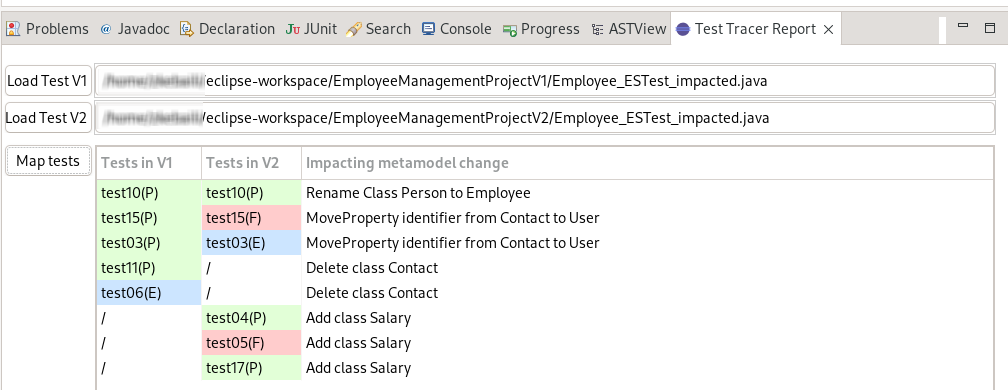
\includegraphics[width=1\textwidth]{./pics/chapter2pics/TestTraceReport.png}
%\caption{Artifacts and structure of a software language in the Eclipse platform.}
\caption{A snippet of the diagnostic report view to visualize and analyze the traced impacted tests.}
\label{fig:toolView}
%\vspace{-5mm}
\end{figure*}